\documentclass{standalone}
\usepackage{tikz}
\usetikzlibrary{arrows.meta, positioning, shapes.geometric, calc,patterns,quotes}

\begin{document}
	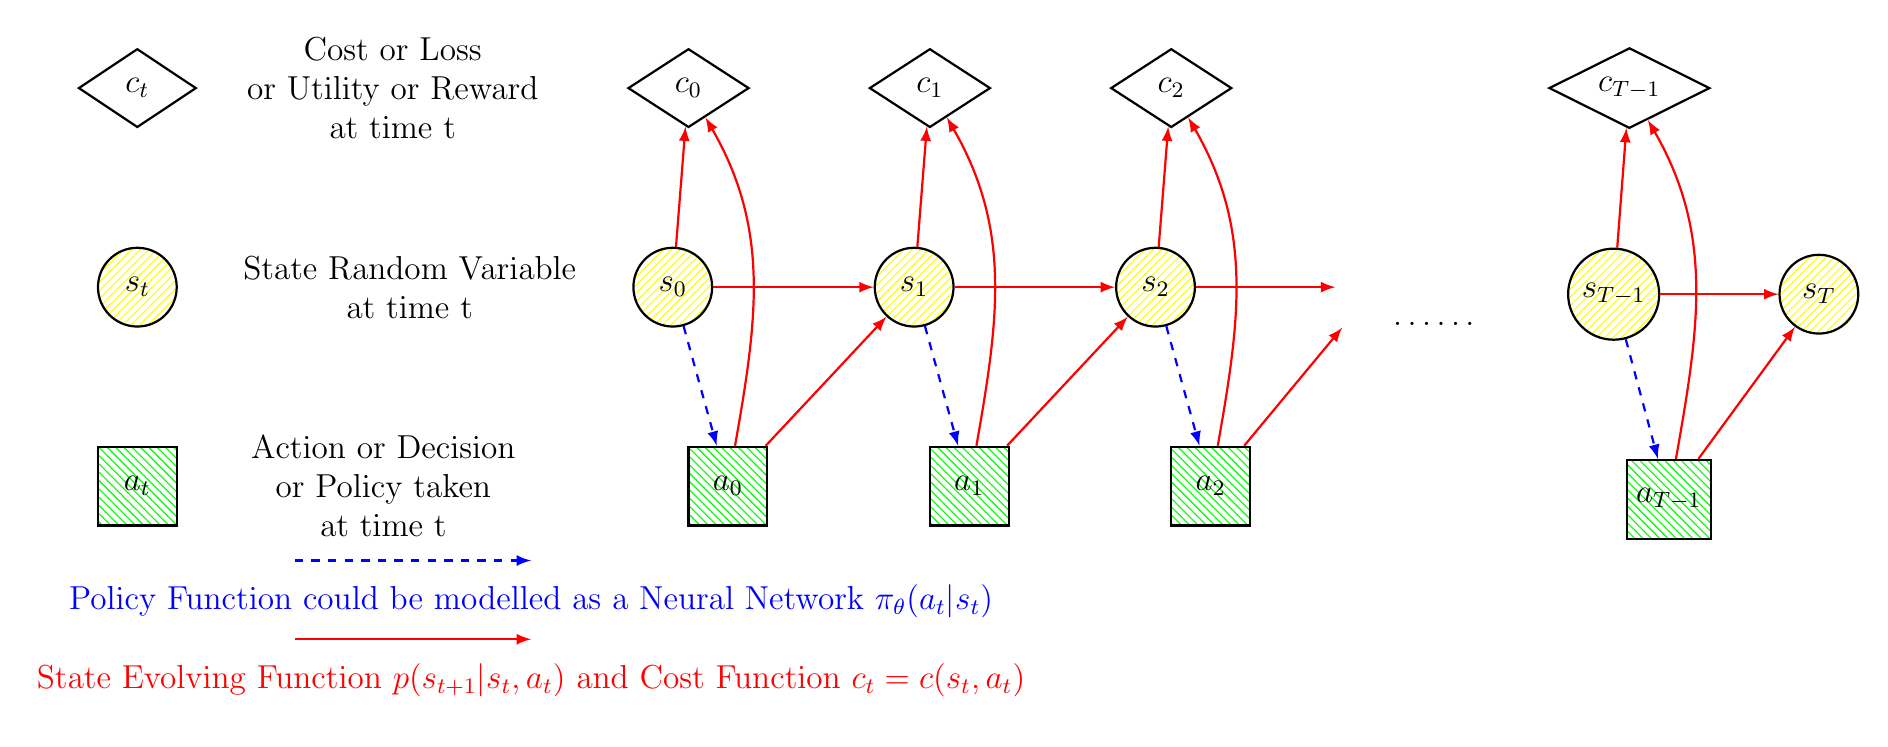
\begin{tikzpicture}[
		node distance=2cm and 1.5cm,
		every node/.style={minimum size=10mm, font=\large},
		cost/.style={draw,diamond, aspect=2, fill=white},
		state/.style={draw,circle,pattern=north east lines, pattern color=yellow},
		obs/.style={draw,circle, fill=white},
		action/.style={draw,rectangle, ,pattern=north west lines, pattern color=green},
		->, >=Stealth, thick, black
		]
		% Nodes for the first stage
		\node[cost] (c0) {$c_0$};
		\node[state, below=of c0, xshift=-2mm, yshift=+5mm] (s0) {$s_0$};
	%	\node[obs, below=of s0, xshift=7mm, yshift=+5mm] (o0) {$o_0$};
		\node[action, below=of s0, xshift=7mm, yshift=+5mm] (a0) {$a_0$};
		% Nodes for the second stage
		\node[cost, right=of c0] (c1) {$c_1$};
		\node[state, below=of c1, xshift=-2mm, yshift=+5mm] (s1) {$s_1$};
	%	\node[obs, below=of s1, xshift=7mm, yshift=+5mm] (o1) {$o_1$};
		\node[action, below=of s1, xshift=7mm, yshift=+5mm] (a1) {$a_1$};
		% Nodes for the third stage
		\node[cost, right=of c1] (c2) {$c_2$};
		\node[state, below=of c2, xshift=-2mm, yshift=+5mm] (s2) {$s_2$};
	%	\node[obs, below=of s2, xshift=7mm, yshift=+5mm] (o2) {$o_2$};
		\node[action, below=of s2, xshift=7mm, yshift=+5mm] (a2) {$a_2$};
		
		% Nodes for the third stage
		\node[draw = white, cost, right=of c2] (c3) {};
		\node[draw = white,fill = white , below=of c3, xshift=-2mm, yshift=+5mm] (s3) {};
	%	\node[draw = white, obs, below=of s3, xshift=7mm, yshift=+5mm] (o3) {};
		\node[draw = white, below=of s3, xshift=7mm, yshift=+5mm] (a3) {};
		% Nodes for the final stage
		\node[cost, right=4cm of c2] (cT1) {$c_{T-1}$};
		\node[state, below=of cT1, xshift=-2mm, yshift=+5mm] (sT1) {$s_{T-1}$};
	%	\node[obs, below=of sT1, xshift=+7mm, yshift=+5mm] (oT1) {$o_{T-1}$};
		\node[state, right=of sT1, xshift=0mm, yshift=0mm] (sT) {$s_T$};
	%	\node[obs, below=of sT, xshift=+7mm, yshift=+5mm] (oT) {$o_T$};
		\node[action, below=of sT1, xshift=7mm, yshift=+5mm] (aT1) {$a_{T-1}$};
		
		\node[draw = white] at (9.5,-3) {\dots \dots};
		
		% Causality arrows
		\draw[-latex,thick,red] (s0) -- (c0);
	%	\draw[-latex,thick,red] (s0) -- (o0);
		\draw[-latex,thick,red] (s0) -- (s1);
		\draw[-latex,thick,red] (a0) to[out=80,in=-60] (c0);
		\draw[-latex,thick,red] (a0) -- (s1);
		\draw[-latex,thick,blue,dashed] (s0) -- (a0);
		%	\draw[-latex,thick,red] (a0) -- (o1);
		%	\draw[-latex,thick,red] (s1) -- (c0);
		% The cost at time step t is affected by the state at time t, at time t+1 and action at time t
		
		% The action at time step t will affect the state at time step t+1, the cost at time step t and the observation at time step t+1
		
		% Causality at second stage
		\draw[-latex,thick,red] (s1) -- (c1);
	%	\draw[-latex,thick,red] (s1) -- (o1);
		\draw[-latex,thick,red] (s1) -- (s2);
		\draw[-latex,thick,red] (a1) to[out=80,in=-60] (c1);
		\draw[-latex,thick,red] (a1) -- (s2);
		\draw[-latex,thick,blue,dashed] (s1) -- (a1);
		%	\draw[-latex,thick,red] (a1) -- (o2);
		%	\draw[-latex,thick,red] (s2) -- (c1);
		
		% Causality at third stage
		\draw[-latex,thick,red] (s2) -- (c2);
	%	\draw[-latex,thick,red] (s2) -- (o2);
		\draw[-latex,thick,red] (s2) -- (s3);
		\draw[-latex,thick,red] (a2) to[out=80,in=-60] (c2);
		\draw[-latex,thick,red] (a2) -- (s3);
		\draw[-latex,thick,blue,dashed] (s2) -- (a2);
		%	\draw[-latex,thick,red] (a2) -- (o3);
		%	\draw[-latex,thick,red] (s3) -- (c2);
		
		% Causality at final stage
		\draw[-latex,thick,red] (sT1) -- (cT1);
	%	\draw[-latex,thick,red] (sT1) -- (oT1);
		\draw[-latex,thick,red] (sT1) -- (sT);
		\draw[-latex,thick,red] (aT1) to[out=80,in=-60] (cT1);
		\draw[-latex,thick,red] (aT1) -- (sT);
		%	\draw[-latex,thick,red] (aT1) -- (oT);
	%	\draw[-latex,thick,red] (sT) -- (oT);
		\draw[-latex,thick,blue,dashed] (sT1) -- (aT1);
		%	\draw[-latex,thick,red] (sT) -- (cT1);
		
		
		% Denote 
		\node[cost] at (-7,0) (costnode) {$c_t$};
		\node[draw = white,right= of costnode,align=center,xshift = -10mm]  {Cost or Loss \\ or Utility or Reward \\at time t};
		\node[state, below = of costnode, yshift = 5mm] (statenode) {$s_t$};
		\node[draw = white, right = of statenode,align = center,xshift = -8mm] {State Random Variable \\ at time t};
		\node[action,below = of statenode,yshift = 5mm]  (actionnode) {$a_t$};
		\node[draw = white, right = of actionnode, align=center,xshift = -7mm] {Action or Decision \\or Policy taken \\ at time t};
		\draw[-latex,thick,blue,dashed] (-5,-6) -- (-2,-6) node[below]{Policy Function could be modelled as a Neural Network $\pi_{\theta}(a_t|s_t)$};
		\draw[-latex,thick,red] (-5,-7) -- (-2,-7) node[below]{State Evolving Function $p(s_{t+1}|s_t,a_t)$ and Cost Function $c_t= c(s_t,a_t)$};
	%	\draw[-latex,thick,red] (6,-7) edge["State Evolving Function and Cost Function"] (10,-7);
		%	\draw[-latex,thick,red] (-7,-11) edge["The given Environment or Reward Function, could be random, but it could be treated as a black box"] (-4,-11);
	\end{tikzpicture}
\end{document}
